\documentclass[12pt]{beamer}
\usepackage{amsmath}
\usepackage[utf8]{inputenc}
\usepackage{apacite}
\usetheme{Singapore}
\usepackage[style=british]{csquotes}

\def\signed #1{{\leavevmode\unskip\nobreak\hfil\penalty50\hskip1em
		\hbox{}\nobreak\hfill #1
		\parfillskip=0pt \finalhyphendemerits=0 \endgraf}}

\newsavebox\mybox
\newenvironment{aquote}[1]
{\savebox\mybox{#1}\begin{quote}\openautoquote\hspace*{-.7ex}}
	{\unskip\closeautoquote\vspace*{1mm}\signed{\usebox\mybox}\end{quote}}

\DeclareMathOperator*{\argmin}{arg\,min}
\usepackage{soul}

\title{Factor Strength and Factor Selection}
\subtitle{An Application to U.S. Stock Market}
\date{\today}
\author[author]{Zhiyuan Jiang\\
			                    28710967\\
[10mm]
			                    {\small Supervisors: Dr Natalia Bailey 
			                    	 \\\hspace{18.5mm} 
			                    	Dr David Frazier}}
		
		
\begin{document}
	
\frame{\titlepage}

%-------------------------------------------------------------------------------------------------------------------------------------------------------------------------------%
%-------------------------------------------------------------------------------------------------------------------------------------------------------------------------------%
\section{Introduction and Motivation}

\begin{frame}{Introduction and Motivation}
Capital Asset Pricing Model (CAPM) is the benchmark of risk pricing.
Assume we have:
\begin{itemize}
\item N asset: i = 1,2,3 $\cdots$ N
\item K risk factors: j = 1,2,3 $\cdots$ K
\item T observation: t = 1,2,3 $\cdots$ T
\end{itemize}
%\[r_{it} - r_{ft} = a_i + \beta_{im}(r_{mt} - r_{ft}) + \sum_{j=1}^{k}\beta_{ij}f_{jt} + \varepsilon_{it} \]
\[r_{it} - rf_{t} = a_i + \beta _{mt}(\bar{r}_{t} - rf_{t}) + \sum_{j=1}^{K}\beta_{ij}f_{jt} + \varepsilon_{it} \]
\frametitle{Motivation}
\begin{columns}
	\begin{column}{0.5\textwidth}
\begin{itemize}
\item $r_{it}$: asset's return
\item $r_{ft}$: risk free return
\item $a_i$: constant/intercept
\item $\beta_{mt}$: market factor loading
%\item $r_{nt}$: asset's return
%\item $rf_{t}$: risk free return
%\item $a_n$: constant/intercept
%\item $\beta _{mt}$: market factor loading
\end{itemize}
	\end{column}
	\begin{column}{0.5\textwidth}  
		\begin{center}
\begin{itemize}
\item $\bar{r}_{t}$: market return 
\item$\beta_{ij}$: risk factor loading
\item $f_{jt}$: risk factor
\item $\varepsilon_{it}$: stochastic error
%\item $\bar{r}_{t}$: market return 
%\item$\beta_{nk}$: risk factor loading
%\item $f_{kt}$: risk factor
%\item $\varepsilon_{nt}$: stochastic error
\end{itemize}
		\end{center}
	\end{column}
\end{columns}
%\begin{itemize}
%\item{\bf Add factors to enhance risk pricing.}
%\item{\bf  New factors are booming }
%\end{itemize}
\end{frame}

\begin{frame}
\frametitle{Why this matters}
CAPM measures the risk and return relationship...\\
\begin{figure}
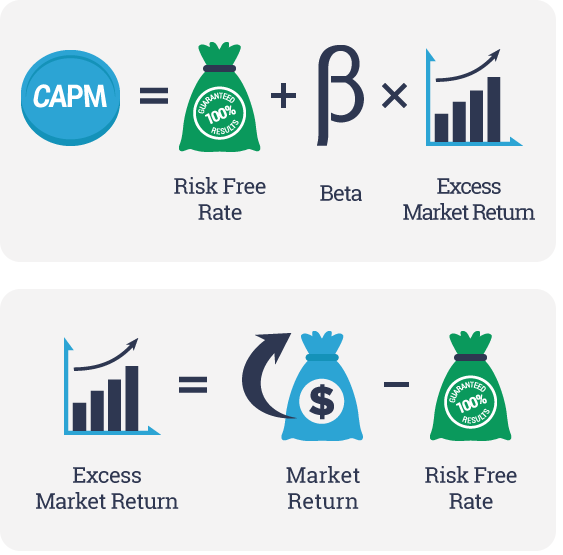
\includegraphics[scale = 0.2]{figure/CAPM.png}
\end{figure}
Fund managers will use this as reference when constructing portfolios.\\
\begin{itemize}
	\item{\bf Add factors to enhance risk pricing.}
	\item{\bf  New factors are booming }
\end{itemize}
\end{frame}

\begin{frame}[plain]
	\begin{figure}
\includegraphics[scale = 0.5]{figure/factor_growth.png}
\caption{Factor amount growing through time. }
	\cite{Harvey2019}\\
	\end{figure}
\end{frame}


\begin{frame}
\frametitle{Problem inside factors}
\begin{enumerate}
	\item  \textbf{Imposters}:
	The significant test is always under some confidence level.
	Some factors appear "significant" purely by chance.
	% With 5\% significance, at least 25 factors will be significant by chance if we have 500 factors.
			\begin{itemize}
%				\item This problem is worse for newly proposed factors \cite{Harvey2014}
                \item	Multiple testing problem
				\item  Can not replicate \cite{Hou2018}
			\end{itemize}
	\item \textbf{Results unreliable}: include "imposters" will distort the estimation
			\begin{itemize}
				\item Statistical inference results unreliable \cite{Gospodinov2017}
				\item Inconsistent estimation \cite{Anatolyev2018}
				\item The portfolio may suffer loss because of this.
			\end{itemize}
\end{enumerate}
\end{frame}

\begin{frame}
\begin{aquote}{\citeNP{Cochrane2011}}
We have a lot of questions to answer: \\
Firstly, which characteristics really provide \textbf{independent} information about average returns? Which are subsumed by others ?
\end{aquote}
	\begin{figure}
	
\includegraphics[scale = 0.2]{figure/cochrane.png}
\end{figure}
\end{frame}

\begin{frame}{Core Problem}
\begin{center}
\alert{\textbf{How to select factors.}}\pause
\end{center}
Numerous methods have been proposed...
\begin{itemize}
\item Solving data mining problem 
\begin{itemize}
\item Bootstrapping \cite{Harvey2015}
\item Bayes method\cite{Barillas2018}
\end{itemize}
\item Machine learning
\begin{itemize}
\item Principle Component Analysis (PCA) \cite{Lettau2020}
\item Lasso\cite{Feng2019}
\end{itemize}
\item $\cdots$
\end{itemize}
\end{frame}



\begin{frame}
	\frametitle{Two Challenges}
	This project faces two challenges:
	\begin{enumerate}
		\item	 High dimensions of risk factor group.\\
		How to identify the significant risk factor. $\Rightarrow$ \alert{use factor strength as criterion.}
		\item 	Correlation among factors \\
		Traditional variable selection algorithm (Lasso) can not handle this.$\Rightarrow$ Will use \alert{elastic net} techniques
	\end{enumerate}
\end{frame}



%-------------------------------------------------------------------------------------------------------------------------------------------------------------------------------%
%-------------------------------------------------------------------------------------------------------------------------------------------------------------------------------%


	\section{Method and Data}
	

	
	\begin{frame}
		\frametitle{Factor Strength}
		Stronger factor $\Rightarrow$ price more asset's risk $\Rightarrow$ generate more significant loadings $\beta$.\\
		Factor strength defined in terms of number of non-zero significant loadings \cite{Bailey2020}.\\
		
		 Assume we have one factor with strength $\alpha_j$:
%		 \begin{itemize}
%\item N assets
%\item J factors
%\item T observation
%		 \end{itemize}
		\begin{align*}
		|\beta_{i}| &> 0,\quad i = 1, 2, 3, \cdots, [N^{\alpha_j}]\\
		|\beta_{i}|&= 0, \quad i = [N^{\alpha_j} ]+1 ,[N^{\alpha_j}]  +2, [N^{\alpha_j}] +3, \cdots, N
		\end{align*}
	
Simply speaking: the more none-zero loadings a factor can generate, the stronger the factor is.
	\end{frame}

\begin{frame}
	For every single risk factor, after running N regression against each assets, we will have a proportion:\\
		\[ \hat{\pi}_j = \frac{\text{Amount of significant non-zero loadings}}{\text{Amount of total loadings/N} }  \]
		\newline
% Proportion	$\hat{\pi_n}$, represent how many non-zero significant loadings are generated.\\
\[\hat{\alpha}_{j}=\left\{\begin{array}{l}
	1+\frac{\ln \hat{\pi}_{ j}}{\ln N}, \text { if } \hat{\pi}_{ j}>0 \\
	0, \text { if } \hat{\pi}_{j} = 0
\end{array}\]
\[ i = 1,2,3,\cdots N,\quad j = 1,2,3, \cdots K\]

$\alpha_j \in [0,1]$.\\
0: no loadings are generate\\
1: the factor has significant non-zero loadings for each assets.
\end{frame}

	
\begin{frame}
\frametitle{Elastic Net}
Introduce by \citeA{Zou2005}, is a modified method to select factor.\\
For demonstration, we consider a simple linear model. $y_i = c + \sum_{j = 1}^K x_{j}\beta_{j}$ \\with N observations: $i = 1,2,3\cdots N$, and K variables.

%$\boldsymbol{y} = c +  \boldsymbol{x}{\boldsymbol{\beta}}$. \\ N observation pairs ($x_i$, $y_i$ ) with $i =1,2,3, \cdots N$, and $\boldsymbol{\beta} = [\beta_1, \beta_2, \beta_3, \cdots, \beta_K]^{\prime}$.

%\[ \hat{\beta} = \argmin\{    \frac{1}{2}[y - x\beta] + \phi P_{\theta}(\beta)        \}   \]
%\[ P_{\theta}(\beta) = (1-\theta)\beta^2 + \theta|\beta|  \]

\[  \hat{\boldsymbol{\beta}} = \argmin \{ \frac{1}{2N}\sum_{i = 1}^N(y_i - c - \sum_{j=1}^{K}\beta_{j}x_{j})^2 + \phi P_\theta(\boldsymbol{\beta})          \}  \]
\[  P_{\theta}(\boldsymbol{\beta}) = \sum_{j = 1}^{K}[(1- \theta)\beta_j^2 + \theta |\beta_j| ]          \]

%\[  \hat{\beta} = \argmin \{ (y_i - c - x_i^{\prime}\beta)^2 + \phi P_\theta(\beta)    \}   \]
%	\[	P_{\theta}(\beta_n) =\sum_{k=1}^K [ (1-\theta)\beta_{nk}^2 + \theta |\beta_{nk}|] \]\\
	
%	\[	\boldsymbol{\hat{\beta}}_{n} = \argmin \{ \frac{1}{2N}\sum_{n = 1}^{N} [r_{nt} - rf_{t}-\hat{a}_{n} -\hat{\beta}_{mt}(\bar{r}_t - rf_t) -\boldsymbol{\hat{\beta}_{n}^{\prime}f_t} ]^2 +\phi P_{\theta}(\boldsymbol{\beta_n})  \} \]
	
%	\[	P_{\theta}(\boldsymbol{\beta_n}) =\sum_{k=1}^K [ (1-\theta)\boldsymbol{\beta}_{nk}^2 + \theta |\boldsymbol{\beta}_{nk}|] \]\\
	
%$\sum_{i = 1}^{N}|\beta_{ij}|$ helps select the factor, reduce redundancy.\\
%$\sum_{i = 1}^{N}\beta_{ij}^2$ helps handle the correlation.
	
%We have to decide two parameter: \alert{$\phi$} and \alert{$\theta$}.
We use the R-package \textbf{\textit{glmnet}}. \cite{Friedman2010}\\
\end{frame}

\begin{frame}
\frametitle{Parameter tuning}
From the loss function, you can see we need to decided on two parameters: \alert{$\phi$} and \alert{$\theta$}.\\
I will not talk about the detail of the parameter tuning just for now...\\
The trick is: minimise the MSE (and cross-validation).\\
\end{frame}


	\begin{frame}
	\frametitle{Data}
	The data set included two parts:
	\begin{itemize}
		\item {\bf Assets}: Standard \& Poor (S\&P) 500 index companies, three year U.S. t-bill, and average market return.\\
		\item {\bf Factor}:  145 factors plus the market factor \\
		
		\item \textbf{Time period}:	Collect thirty years data: 1988:1-2017:12.\\
		
		\item We focusing on the thirty year data, but also use 10/20 year data set to see how the factor strength eveolove.\\
	\end{itemize}		\\

	\resizebox{\textwidth}{!}{	
		\begin{tabular}{c|ccc}
			\hline
			& Time Span                    & Number of Companies (n) & Observations Amount (T) \\ \hline
%			10 Years & January 2008 - December 2017 & 419                  & 120                     \\
%			20 Years & January 1998 - December 2017 & 342                  & 240                     \\
			30 Years & January 1988 - December 2017 & 242                  & 360                     \\ \hline
	\end{tabular}}
\end{frame}

\section{Empirical Findings}

\begin{frame}[plain]
\frametitle{Proportion of factors with strength falling into different range (145 risk factors)}
\begin{figure}
        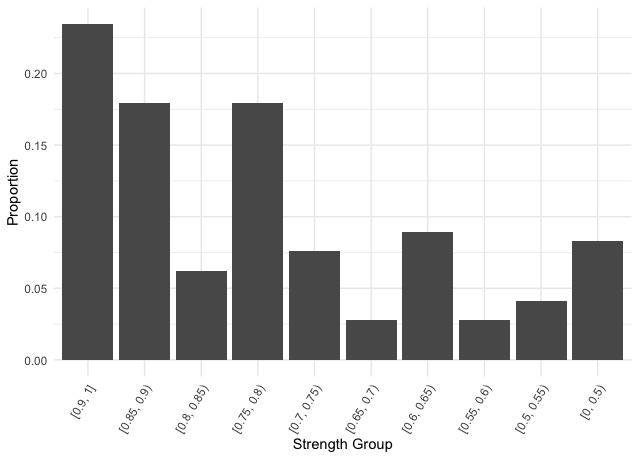
\includegraphics[scale = 0.45]{figure/30_strength.png}
\end{figure}
\end{frame}


%\begin{frame}
%	\frametitle{Top 10 strong factors and three famous factors}
%\resizebox{\textwidth}{!}{
%	\begin{tabular}{llc|llc|llc}
%	\hline
%	\multicolumn{3}{c|}{Ten Year} & \multicolumn{3}{c|}{Twenty Yera} & \multicolumn{3}{c}{Thirty Year} \\ \hline
%	Rank & Factor     & Strength & Rank   & Factor     & Strength   & Rank   & Factor     & Strength   \\ \hline
%	 	 & Market & 0.988 & &Market & 0.990 & &Market & 0.995 \\
%	1   & beta               & 0.749    & 1      & ndp           & 0.937      & 1      & salecash  & 0.948\\
%	2   & baspread       & 0.730    & 2      & quick        & 0.934      & 2      & ndp          & 0.941\\
%	3   & turn               & 0.728    & 3      & salecash   & 0.933      & 3      & quick      & 0.940\\
%	4   & zerotrade      & 0.725    & 4      & lev            & 0.931      & 4      & age         & 0.940\\
%	5   & idiovol           & 0.723    & 5      & cash         & 0.931      & 5      & roavol    & 0.938\\
%	6   & retvol            & 0.721    & 6      & dy             & 0.929      & 6      & ep           & 0.937\\
%	7   & std\_turn      & 0.719    & 7      & roavol      & 0.929      & 7      & depr       & 0.935\\
%8   & HML\_Devil & 0.719    & 8      & zs              & 0.927      & 8      & cash       & 0.934\\
%	9   & maret           & 0.715    & 9        & age          & 0.927      & 9      & rds         & 0.931\\
%	10 & roavol          & 0.713    & 10     & cp             & 0.926      & 10    & dy          & 0.927 \\
%	20 & UMD            & 0.678    & 29     & HML        & 0.905      & 39     & HML       & 0.894 \\
%	24 & HML            & 0.672    & 76     & SMB        & 0.770      & 68     & SMB        & 0.804 \\
%	87 & SMB            & 0.512    & 89     & UMD        & 0.733      & 96     & UMD       & 0.745 \\ 
%	\hline
%\end{tabular}
%}
%\end{frame}


\begin{frame}[shrink = 20]
		\frametitle{Top 10 strongest factors and three famous factors}
\begin{center}
	\begin{tabular}{lll}
	
	\hline
	\multicolumn{3}{c}{Thirty Year} \\ \hline
	Rank   & Factor     & Strength  \\ \hline
	& Market     & 0.995     \\
	1      & salecash   & 0.948     \\
	2      & ndp        & 0.941     \\
	3      & quick      & 0.940     \\
	4      & age        & 0.940     \\
	5      & roavol     & 0.938     \\
	6      & ep         & 0.937     \\
	7      & depr       & 0.935     \\
	8      & cash       & 0.934     \\
	9      & rds        & 0.931     \\
	10     & dy         & 0.927     \\
	39     & HML        & 0.894     \\
	68     & SMB        & 0.804     \\
	96     & UMD        & 0.745     \\ 
	\hline
\end{tabular}
\end{center}


\end{frame}


\begin{frame}[plain]
	\frametitle{Correlation of Factors: from strong to weak}
	\begin{figure}
		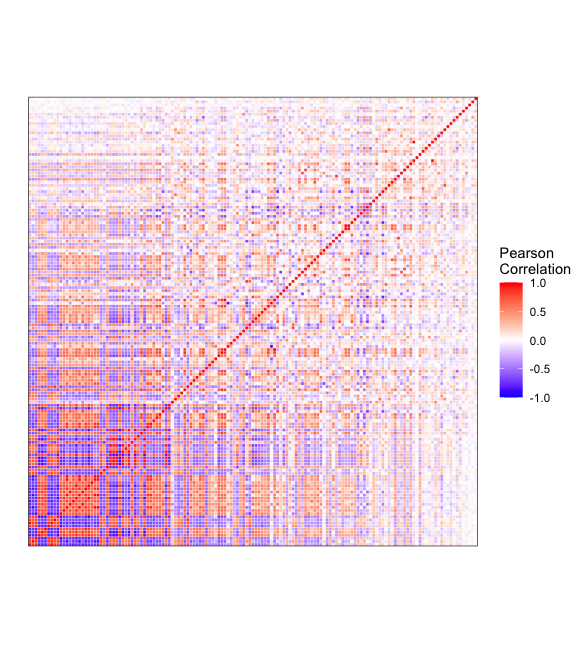
\includegraphics[scale = 0.4]{figure/correlation_heat_map.png}
	\end{figure}
\end{frame}


\begin{frame}
\frametitle{Correlation among factors.}
\resizebox{\textwidth}{!}{
	\begin{tabular}{l|cccccc}
		\hline
		\hline
		Factor Group                                 & [0,0.5{)} & [0.5, 0.6{)} & [0.6, 0.7{)} & [0.7, 0.8{)} & [0.8,0.9{)} & [0.9,1{]} \\ \hline
		\multicolumn{1}{c|}{Correlation Coefficient} & 0.0952    & 0.157        & 0.213        & 0.229        & 0.371       & 0.724   \\
		Factor Amount &12 & 10 &  17 & 37& 35 &34  \\ \hline \hline
	\end{tabular}\\
}

\begin{itemize}
\item Correlation among strong factor is very high.
\item Among weak factors is very low.
\item  Recall the problem Lasso can not handle correlation...
\end{itemize}
\end{frame}



\begin{frame}
	\frametitle{Factor Selection Result}
	\resizebox{\textwidth}{!}{

			\begin{tabular}{l|ccccccc}
			\hline
			\hline
Factor Group                                     & [0,0.5{)} & [0.5, 0.6{)} & [0.6, 0.7{)} & [0.7, 0.8{)} & [0.8,0.9{)} & [0.9,1{]} & mix \\ 
			Factor Amount                  & 12            & 10               & 17               & 37               & 35              & 34            & 20  \\ \hline
			\begin{tabular}[c]{@{}c@{}}Proportion of Agreement\\ (Exact)\end{tabular} & \alert{68.7\%}                        & 55.9\%                           & 42.8\%                           & 20.9\%                           & 17.7\%                          & \alert{13.9\%}                        & 34.6\% \\
			\begin{tabular}[c]{@{}c@{}}Proportion of Agreement\\ (90\%)\end{tabular}  & 86.8\%                        & 72.0\%                           & 74.5\%                           & 72.0\%                           & 79.8\%                          & 74.4\%                        & 76.1\% \\\hline
		Avg EN selection amount        & \alert{2.11}          & 4.47             & 8.67             & 14.67            & 13.51           & \alert{12.37}         & 8.45                  \\
		Avg EN selection proportion    & 17.5\%        & 44.73\%          & 51.00\%          & 39.65\%          & 38.61\%         & 36.38\%       & 42.28\%                 \\
		Avg Lasso selection amount     & \alert{2.06}          & 3.87             & 8.43             & 13               & 12.19           & \alert{10.46}         & 7.26                    \\
		Avg Lasso selection proportion & 17.2\%        & 38.76\%          & 49.60\%          & 35.14\%          & 34.83\%         & 30.75\%       & 36.27\%                 \\ \hline\hline
	\end{tabular}
}
\begin{itemize}
\item Agreement decrease with factor strength increase
\item	Lasso produce parsimonious model
\item	When facing weak factors, both Lasso and EN can well reduce redundancy.
\item Eight of Top 10 most selected factors from mix factor group are strong factors.
\end{itemize}
\end{frame}

%-------------------------------------------------------------------------------------------------------------------------------------------------------------------------------%
%-------------------------------------------------------------------------------------------------------------------------------------------------------------------------------%


\section*{epilogue}
\begin{frame}
\frametitle{Wrap Up}
\begin{itemize}
\item 
\item Elastic net doing pretty well on eliminating weak factors.
\item MSE is not a good criterion for finance when tuning parameters.
\end{itemize}
\end{frame}

\begin{frame}
\frametitle{Potential Extension}
\begin{enumerate}
\item Using other criterion for tuning parameter
\item Categorised the factors and stocks
\item Using other methods to select factors, compare with the Lasso and Elastic net.
\end{enumerate}
\end{frame}


\begin{frame}
	\centering	
\huge{ Thanks for listening\\}
\end{frame}

	\section*{}
\begin{frame}
\frametitle{EN parameter tuning}
Recall our simple toy multi-variables regression: $\boldsymbol{y} = c +  \boldsymbol{x}{\boldsymbol{\beta}}$. \\ N observation pairs ($x_i$, $y_i$ ) with $i =1,2,3, \cdots N$, and $\boldsymbol{\beta} = [\beta_1, \beta_2, \beta_3, \cdots, \beta_K]^{\prime}$.
\[  \hat{\boldsymbol{\beta}} = \argmin \{ \sum_{i = 1}^N(y_i - c - \sum_{j=1}^{K}\beta_{j}x_{ij})^2 + \phi P_\theta(\boldsymbol{\beta})          \}  \]
\[  P_{\theta}(\boldsymbol{\beta}) = \sum_{j = 1}^{K}[(1- \theta)\beta_j^2 + \theta |\beta_j| ]          \]
%\[	\boldsymbol{\hat{\beta}}_{i} = \argmin \{ \frac{1}{2N} (x_{it}-\hat{a}_{iT} - \boldsymbol{\hat{\beta}_{i}^{\prime}f_t}^2 ) +\phi P_{\theta}(\boldsymbol{\beta_i})  \} \]

%\[	P_{\theta}(\boldsymbol{\beta_i}) =\sum_{j=1}^k [ (1-\theta)\boldsymbol{\beta}_{ij}^2 + \theta |\boldsymbol{\beta}_{ij}|] \] \\
The R package \textbf{\textit{glmnet}} provides function to tuning parameter $\phi$, using cross-validation, targeting at minimise the MSE.\\
We use the same principle: minimise the MSE to determine our $\theta$ value.\\
\end{frame}

	\section*{}
\begin{frame}
Assume we have N units of stock, J risk factors, and T observations.\\
\begin{enumerate}
\item Assign first 90\% of data as learning set, and rest 10\% as test set.
\item Prepare a sequence of $\theta$ values, from 0 to 1, with step 0.01
\item For each $\theta$, we use the learning set to fit a model, with $\phi$ selected by the function
\item Base on the fitted model, makes prediction and compare with the test set, and calculate the MSE.
\item The $\theta-\phi$ combination with smallest MSE is the winner.
\end{enumerate}
\end{frame}

	\section*{}
\begin{frame}
In practice, because the problem of computation burden, we will randomly select 10 factors from each group, and 10 companies to conduct the procedure.\\
Then, we repeat the whole procedure 2000 times, and take the average of parameter results.\\ 
\end{frame}


%-------------------------------------------------------------------------------------------------------------------------------------------------------------------------------%
%-------------------------------------------------------------------------------------------------------------------------------------------------------------------------------%
\begin{frame}[allowframebreaks]
	\frametitle{Bibliography}
	\bibliographystyle{apacite}
{\footnotesize\bibliography{library.bib}}
\end{frame}
\end{document}